\documentclass[crop,tikz]{standalone}

\usetikzlibrary{shapes,arrows,matrix,positioning,external}
\newcommand*{\h}{\hspace{5pt}}% for indentation
\newcommand*{\hh}{\h\h}% double indentation
\usepackage{mathpazo}

\begin{document}

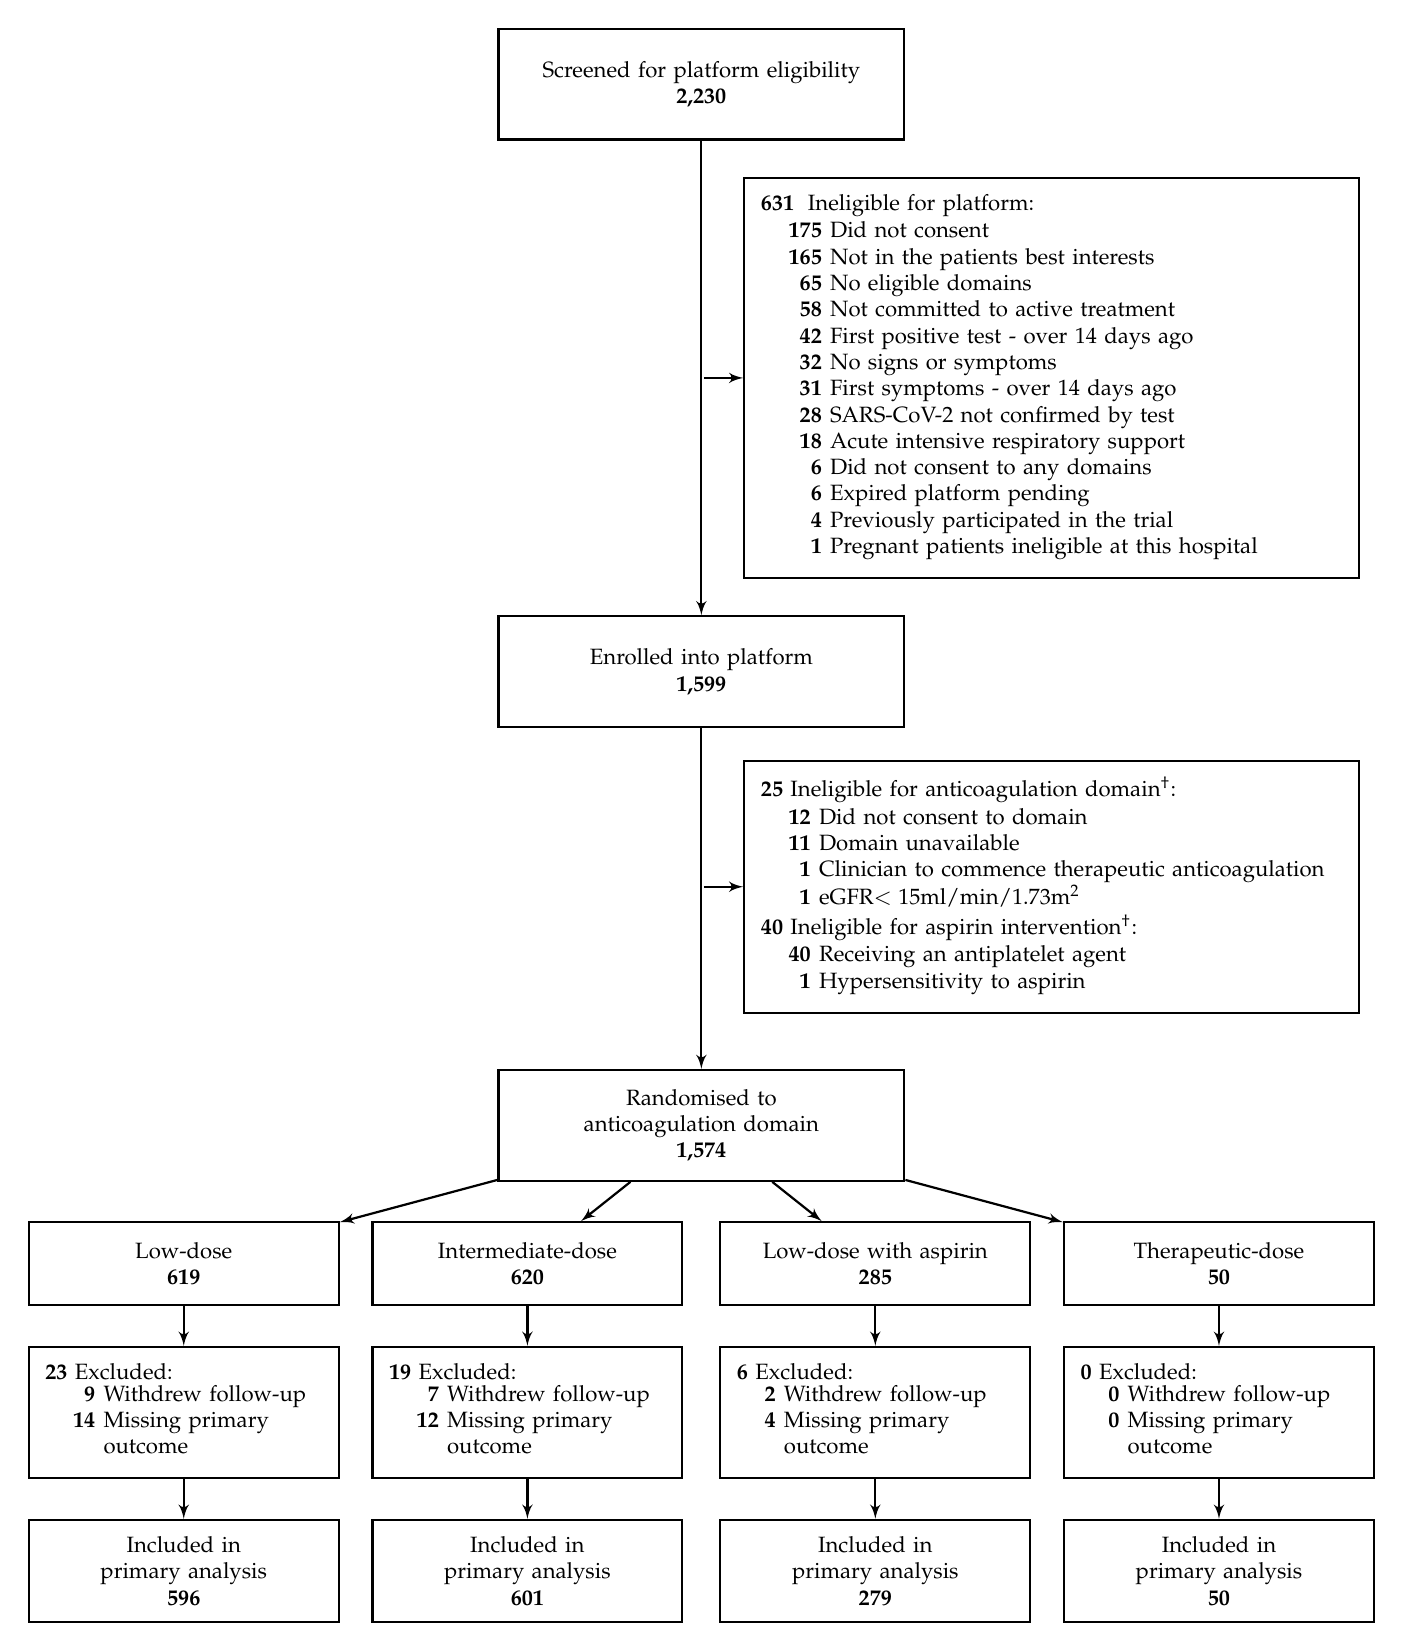
\begin{tikzpicture}[auto,
    block_center/.style ={rectangle, draw=black, thick, fill=white, font = \footnotesize,
      text width=14em, text centered, minimum height=4em},
    block_assign/.style ={rectangle, draw=black, thick, fill=white, anchor=north, font = \footnotesize,
      text width=10em, text centered, minimum height=3em, inner sep=6pt},
    block_left/.style ={rectangle, draw=black, thick, fill=white, font = \footnotesize,
      text width=21em, text ragged, minimum height=4em, inner sep=6pt},
    block_left_small/.style ={rectangle, draw=black, thick, fill=white, font = \footnotesize,
      text width=10em, text ragged, minimum height=2em, inner sep=6pt},
    block_blank/.style={rectangle, draw=white, thick, fill=white, font = \footnotesize,
      text width=0em, text ragged, minimum height=0em, inner sep=0pt},
    block_noborder/.style ={rectangle, draw=none, thick, fill=none, font = \footnotesize,
      text width=10em, text centered, minimum height=0.5cm},
    line/.style ={draw, thick, -latex', shorten >=0pt}]
    % row
    \node [block_center] (screened) {Screened for platform eligibility\\ \textbf{2,230}};
   \node [block_blank] (blank0) [below=3cm of screened] {};
   \node [block_left] (pineligible) [right=0.5cm of blank0] {\textbf{631}\h Ineligible for platform: \\
     \begin{tabular}{@{\hskip 10pt}r@{\hskip 3pt}l}
       \textbf{175} & Did not consent \\
       \textbf{165} & Not in the patients best interests \\
       \textbf{65} & No eligible domains \\
       \textbf{58} & Not committed to active treatment \\
       \textbf{42} & First positive test - over 14 days ago \\
       \textbf{32} & No signs or symptoms \\
       \textbf{31} & First symptoms - over 14 days ago \\
       \textbf{28} & SARS-CoV-2 not confirmed by test \\
       \textbf{18} & Acute intensive respiratory support \\
       \textbf{6} & Did not consent to any domains \\
       \textbf{6} & Expired platform pending \\
       \textbf{4} & Previously participated in the trial \\
       \textbf{1} & Pregnant patients ineligible at this hospital
     \end{tabular}};
    \node [block_center] (peligible) [below=3cm of blank0] {Enrolled into platform\\ \textbf{1,599}};
    \node [block_blank] (blank1) [below=2cm of peligible] {};
    \node [block_left] (ineligible) [right=0.5cm of blank1] {\textbf{25} Ineligible for anticoagulation domain\textsuperscript{$\dagger$}: \\
    \begin{tabular}{@{\hskip 10pt}r@{\hskip 3pt}l}
      \textbf{12} & Did not consent to domain \\
      \textbf{11} & Domain unavailable \\
      \textbf{1} & Clinician to commence therapeutic anticoagulation \\
      \textbf{1} & eGFR$<15$ml/min/$1.73$m\textsuperscript{$2$}
    \end{tabular} \\
    \textbf{40} Ineligible for aspirin intervention\textsuperscript{$\dagger$}: \\
    \begin{tabular}{@{\hskip 10pt}r@{\hskip 3pt}l}
      \textbf{40} & Receiving an antiplatelet agent \\
      \textbf{1} & Hypersensitivity to aspirin
    \end{tabular} };
    % row 3
    \node [block_center] (randomised) [below = 2.3cm of blank1] {Randomised to \\ anticoagulation domain\\ \textbf{1,574}};
    % row 4
    \node [block_assign] (int0) [below left=0.5cm and 2cm of randomised] {Low-dose \\ \textbf{619}};
    \node [block_assign] (int1) [right=0.4cm of int0] {Intermediate-dose \\ \textbf{620}};
    \node [block_assign] (int3) [below right=0.5cm and 2cm of randomised] {Therapeutic-dose \\ \textbf{50}};
    \node [block_assign] (int2) [left=0.4cm of int3] {Low-dose with aspirin \\ \textbf{285}};
    % row 5
    \node [block_left_small] (int0excl) [below = 0.5cm of int0] {\textbf{23} Excluded: \\
    \begin{tabular}{@{\hskip 10pt}r@{\hskip 3pt}l}
      \textbf{9}  & Withdrew follow-up \\
      \textbf{14} & Missing primary \\
                  & outcome
    \end{tabular}};
    \node [block_left_small] (int1excl) [below = 0.5cm of int1] {\textbf{19} Excluded: \\
    \begin{tabular}{@{\hskip 10pt}r@{\hskip 3pt}l}
      \textbf{7}  & Withdrew follow-up \\
      \textbf{12} & Missing primary \\
                  & outcome
    \end{tabular}};
    \node [block_left_small] (int2excl) [below = 0.5cm of int2] {\textbf{6} Excluded: \\
    \begin{tabular}{@{\hskip 10pt}r@{\hskip 3pt}l}
      \textbf{2} & Withdrew follow-up \\
      \textbf{4} & Missing primary \\
                 & outcome
    \end{tabular}};
    \node [block_left_small] (int3excl) [below = 0.5cm of int3] {\textbf{0} Excluded: \\
    \begin{tabular}{@{\hskip 10pt}r@{\hskip 3pt}l}
      \textbf{0} & Withdrew follow-up \\
      \textbf{0} & Missing primary \\
                 & outcome
    \end{tabular}};
    % row
    \node [block_assign] (int0analysis) [below = 0.5cm of int0excl] {Included in\\ primary analysis \\ \textbf{596}};
    \node [block_assign] (int1analysis) [below = 0.5cm of int1excl] {Included in\\ primary analysis \\ \textbf{601}};
    \node [block_assign] (int2analysis) [below = 0.5cm of int2excl] {Included in\\ primary analysis \\ \textbf{279}};
    \node [block_assign] (int3analysis) [below = 0.5cm of int3excl] {Included in\\ primary analysis \\ \textbf{50}};
    % connecting nodes with paths
    \begin{scope}[every path/.style=line]
      \path (screened)   -- (peligible);
      \path (blank0)     -- (pineligible);
      \path (peligible)  -- (randomised);
      \path (blank1)     -- (ineligible);
      \path (randomised) -- (int0);
      \path (randomised) -- (int1);
      \path (randomised) -- (int2);
      \path (randomised) -- (int3);
      \path (int0) -- (int0excl);
      \path (int1) -- (int1excl);
      \path (int2) -- (int2excl);
      \path (int3) -- (int3excl);
      \path (int0excl) -- (int0analysis);
      \path (int1excl) -- (int1analysis);
      \path (int2excl) -- (int2analysis);
      \path (int3excl) -- (int3analysis);
    \end{scope}
  \end{tikzpicture}


\end{document}
